\documentclass[12pt, a4paper]{ctexart}


\usepackage{ctex}
\usepackage{amsmath}
\usepackage{amssymb}
\usepackage{amsthm}
\usepackage{geometry}
\usepackage{graphicx}
\geometry{a4paper,left=2cm,right=2cm,top=2.5cm,bottom=2cm}
\newenvironment{prooff}{{\noindent\it\textcolor{cyan!40!black}{Proof}:}\quad}{\par}
\usepackage[dvipsnames]{xcolor}
\usepackage{tcolorbox}
\usepackage{enumerate}
\usepackage{cite}
\usepackage[colorlinks,linkcolor=cyan!40!black]{hyperref}
\usepackage{tikz}
\usepackage{setspace}

\newcommand{\bbrace}[1]{\left\{ #1 \right\} }
\newcommand{\bb}[1]{$\mathbb{#1}$}
\newcommand{\p}{^{\prime}}
\renewcommand{\mod}[1]{(\text{mod}\,#1)}


\newcounter{exercise}
\renewcommand{\theexercise}{\text{习题\,}\stepcounter{exercise}\arabic{exercise}}
\newcounter{subexercise}[exercise]
\renewcommand{\thesubexercise}{\stepcounter{subexercise}(\alph{subexercise})}

\newtheorem{lem}{Lemma}[section]
\newtheorem{prop}{Proposition}[section]
\newtheorem{defn}{Definition}[section]
\newtheorem{coro}{Corollary}[section]
\newtheorem{theo}{Theorem}[section]
\newtheorem{exer}{Exercise}[subsection]
%\arabic{exercise}显示计时器的值
\title{冯克勤《代数数论》题解与勘误}
\author{尔濯}
\date{}
\begin{document}
\thispagestyle{empty}
\maketitle
% \begin{center}
%     \,\\
%     \vskip 2cm
%     \fontsize{30}{18}
%     \textbf{冯克勤《代数数论》题解与勘误}\\
%     \vskip 1.5cm
%     \kaishu \fontsize{20}{18}
%     尔濯
% \end{center}

% \tikz[remember picture,overlay] \node[opacity=0.7,inner sep=0pt] at (current page.center){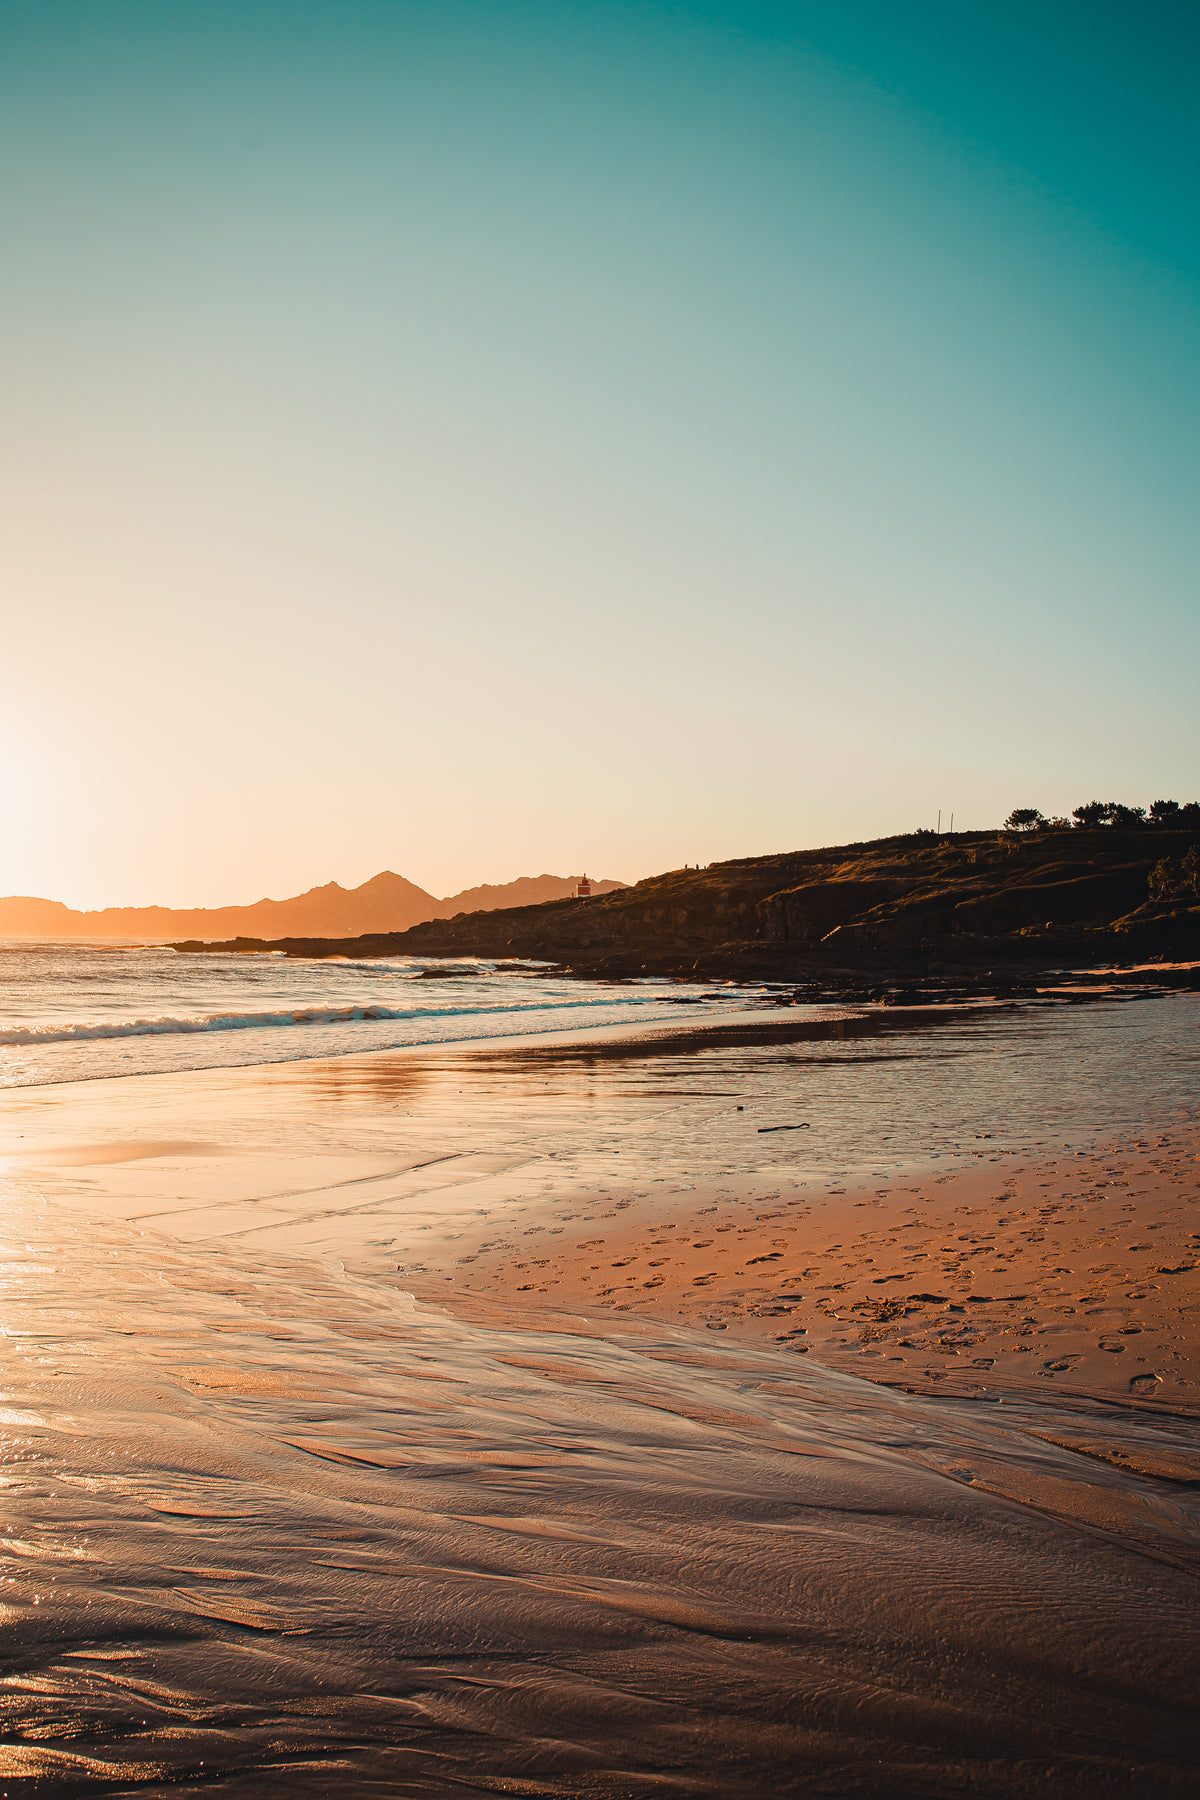
\includegraphics[width=\paperwidth,height=\paperheight]{background.jpg}};
\tableofcontents
\newpage
\section{代数数域和代数整数环}
\subsection{代数数域}

% \begin{tcolorbox}[colback=Emerald!10,colframe=cyan!40!black,title=\theexercise]
%     代数数集合是可数的,超越数集合是不可数的。
% \end{tcolorbox}
\begin{exer}
    代数数集合是可数的,超越数集合是不可数的。
\end{exer}
\begin{prooff}
    用$I$表示所有整系数多项式之集,$A_i$表示$i\in I$的所有根组成的集合,
    则全体代数数集合$A$可以表为:
    \begin{equation*}
        A=\bbrace{\alpha:\alpha \text{为某个整系数多项式的根}}=\bigcup_{i\in I}A_i
    \end{equation*}
    显然$A_i$为有限集进而为可数集,如果我们证明全体整系数多项式之集可数,那么全体代数数可数。


    记第$n$个素数为$p_{n-1}$,我们去证明$I$到$\mathbb{Z}_{>0}$有一个单射。
    考虑映射:\begin{equation*}
        a_nx^n+\dots+a_1x+a_0 \rightarrow \prod_{i=0}^{n}p_i^{f(a_i)}
    \end{equation*}
    其中
    \begin{equation*}
        f(x)=\begin{cases}
            2x \qquad x>0 \\
            1-2x\qquad x\le 0
        \end{cases}
    \end{equation*}
    这显然是单射,从而证明了代数数可数,假如超越数也可数,与\bb{R}不可数矛盾。
\end{prooff}
\begin{exer}
    (a)每个二次数域都可以表成$\mathbb{Q}(\sqrt{d})$,其中$d$为无平方因子整数。\\
    (b)如果$d,d\p$为不同的无平方因子整数,则$\mathbb{Q}(\sqrt{d})\neq\mathbb{Q}(\sqrt{d\p})$\\
    (c)二次数域必为有理数域的伽罗瓦扩张,试求其伽罗瓦群。\\
\end{exer}


\begin{prooff}
    在二次数域$K$中取一个与$1$线性无关的数$\alpha$,考虑其最小多项式为二次首一有理系数多项式,用求根公式将$\alpha$解出得到:
    \begin{equation*}
        \alpha=a+b\sqrt{d},\quad a,b\in \mathbb{Q},d\in \mathbb{Z}
    \end{equation*}
    从而不难证明:\bb{Q}$(\sqrt{d})=K$


    如果$\mathbb{Q}(\sqrt{d})=\mathbb{Q}(\sqrt{d\p})$
    那么$\sqrt{d}=a+b\sqrt{d\p}\quad a,b\in \mathbb{Q}$,平方以后得到$a=0$,从而推出$m\sqrt{d}=n\sqrt{d\p},\quad m,n\in \mathbb{Z}$
    ,平方后比较两边$d,d\p$素因子幂次,借助无平方因子,得到$d=d\p$。

    再考虑一个二次数域$K=\mathbb{Q}(\sqrt{d})$,由于$\sqrt{d}\rightarrow \pm \sqrt{d}$诱导出来两个不同的$K$的自同构,所以\text{Galois}群为二阶循环群。
\end{prooff}
\begin{exer}
    (a) 求下列代数数的次数和最小多项式:
    \begin{equation*}
        \sqrt{2}+\sqrt{3}+\sqrt{5},\sqrt{2+\sqrt{2}},\sqrt{2}+e^{2\pi\text{i}/3}
    \end{equation*}
    (b)求$\sqrt{2}+\sqrt{3}+\sqrt{5}$在$\mathbb{Q}(\sqrt{30})$的共轭元。
\end{exer}
\begin{prooff}
    $\sqrt{2+\sqrt{2}}$显然是$f_2(x)=x^4-4x^2+2$的根(由两次平方得来),而$f_2(x)$由爱森斯坦判别法是不可约多项式,因此是其最小多项式。

    对于$\sqrt{2}+\sqrt{3}+\sqrt{5}$,可以通过移项和平方构造出一个8次多项式使其以$\sqrt{2}+\sqrt{3}+\sqrt{5}$作为根,现在我们证明:
    \begin{equation*}
        [\mathbb{Q}(\sqrt{2}+\sqrt{3}+\sqrt{5}):\mathbb{Q}]=8
    \end{equation*}
    由此可以得到需要的结论,这需要一个引理:
    \begin{lem}
        $p_1,\dots,p_n$为不同素数,则:
        \begin{equation*}
            [\mathbb{Q}(\sqrt{p_1},\dots,\sqrt{p_n}):\mathbb{Q}]=2^n
        \end{equation*}
        \label{lem1.1}
    \end{lem}
    这个引理蕴含着$p_1,\dots,p_n$的任意子集的乘积(共$2^n$个,空集视为$1$)在\bb{Q}上的线性无关性。
    我们用归纳法证明一个更强的结论:$A=\bbrace{x_1,\dots,x_n}$是\bb{Z}的子集使得任意$A$的非空子集的元素相乘不为\bb{Z}中平方元,则:
    \begin{equation*}
        [\mathbb{Q}(\sqrt{x_1},\dots,\sqrt{x_n}):\mathbb{Q}]=2^n
    \end{equation*}
    $n=1$时显然,$n=2$时,$[\mathbb{Q}(\sqrt{x_1},\sqrt{x_2}):\mathbb{Q}]=[\mathbb{Q}(\sqrt{x_1},\sqrt{x_2}):\mathbb{Q}(\sqrt{x_2})][\mathbb{Q}(\sqrt{x_2}):\mathbb{Q}]$
    只需证明:$[\mathbb{Q}(\sqrt{x_1},\sqrt{x_2}):\mathbb{Q}(\sqrt{x_2})]=2$,假如$\sqrt{x_1}=a+b\sqrt{x_2},\quad a,b\in \mathbb{Q},b=\frac{p}{q}$,平方后得到$a=0$,从而有:
    $q^2x_1x_2=p^2x_2^2$,左边必有一个素因子幂次为奇数,矛盾。

    用归纳法,假设对所有$<n$的数成立,$n\ge 3$。

    设$L= \mathbb{Q}(\sqrt{p_1},\dots,\sqrt{p_{n-2}})$,则由归纳假设只需证明:
    $[L(\sqrt{x_{n-1}},\sqrt{x_n}):L]=4$,
    如果$\sqrt{x_{n-1}},\sqrt{x_n},\sqrt{x_{n-1}x_n}$之中有$\in L$的元素,则会与$n-1$时的结论矛盾。
    因此$[L(\sqrt{x_{n-1}},\sqrt{x_n}):L]=2[L(\sqrt{x_{n-1}},\sqrt{x_n}):L(\sqrt{x_{n-1}}]$,而如果$\sqrt{x_n}=l_1+l_2\sqrt{x_{n=1}}$,移向平方后与$\sqrt{x_nx_{n-1}}\notin L$矛盾,从而我们完成了引理的证明。

    令$x=\sqrt{2}+\sqrt{3}+\sqrt{5}$,移向平方两次可以得到$\mathbb{Q}(\sqrt{2}+\sqrt{3}+\sqrt{5})\supseteq \mathbb{Q}(\sqrt{30}) $,因此只需证明:
    $[\mathbb{Q}(\sqrt{2}+\sqrt{3}+\sqrt{5}):\mathbb{Q}(\sqrt{30})]=4$

    事实上$\sqrt{2}+\sqrt{3}+\sqrt{5}$是$x^4-20x^2-8\sqrt{30}x-24$的根,而如果他还是$\mathbb{Q}(\sqrt{30})$上一个二次多项式的根(扩张次数只能是二的幂),将多项式设出来,然后利用引理得到的线性无关性可得该待定系数得到的方程无解,从而$x^4-20x^2-8\sqrt{30}x-24$是
    $\sqrt{2}+\sqrt{3}+\sqrt{5}$在$\mathbb{Q}(\sqrt{30})$上的最小多项式,这也完成了第二问的证明,即共轭元素为$x^4-20x^2-8\sqrt{30}x-24$的四个根。


    令$c=\sqrt{2}+e^{2\pi\text{i}/3}$,计算得知$\sqrt{2}=\frac{c^2+c+3}{1+2c}$,从而$[\mathbb{Q}(c):\mathbb{Q}]=[\mathbb{Q}(c):\mathbb{Q}(\sqrt{2})][\mathbb{Q}(\sqrt{2}):\mathbb{Q}]=4$
    ,上式成立只需注意到$c$为虚数故前者不可能为$1$

    因此,$(x^2+x+3)^2-2(1+2x)^2$为其最小多项式

\end{prooff}
\begin{exer}
    全体代数数构成域,且为有理数域的无限次扩张。
\end{exer}

\begin{prooff}
    前一个命题是域论基本结论,可以参考\cite{dummit1991abstract}的Chapter\,$13$。
    后者只需注意到由爱森斯坦判别法,对于任意正整数$n$,\,$x^n-2$为$\mathbb{Q}[x]$上不可约多项式,从而:
    $\bbrace{(\sqrt[n]{2})^a:0\le a\le n-1 }$在\bb{Q}上线性无关。
\end{prooff}
\begin{exer}
    一个代数整数是单位根的充要条件是每个共轭元素模长为1
\end{exer}
\begin{prooff}
    该证明参考了MSE上的讨论:
    \url{https://math.stackexchange.com/questions/4323}


    只证明全部共轭元素模长为$1$则为单位根,另一边是显然的。


    对于代数整数$\alpha$,设其最小多项式为:$f(x)=x^n+\dots+a_1x+a_0$,其中$a_i\in$\bb{Z},设其全部共轭元素为$\alpha_1,\dots,\alpha_n$,其中$\alpha=\alpha_1$,
    则$f(x)=\prod_{i=1}^{n}(x-\alpha_i)$,再考虑一列多项式$f_m(x)=\prod_{i=1}^{n}(x-\alpha_i^m)$,由韦达定理,每个根都模长为$1$的$n$次整系数多项式的每个系数有上界(只与$n$有关),因此只有有限多个每个根都模长为$1$的$n$次整系数多项式。
    考虑对称多项式基本定理\cite{丘维生},$f_m(x)$均为整系数多项式,因此在$f_m(x)$中取出任意多项(不妨取$n+1$项)使得他们表示同一个多项式,对比这些项的根,如果第一项为$f_s(x)$,则有根$\alpha^s$,之后$n$项里面,要么有$\alpha^t$使得$\alpha^t=\alpha^t$,此时$\alpha$
    已经为单位根,要么由抽屉原理有$\alpha^s=\alpha_i^{t_1}=\alpha_i^{t_2}$,此时$\alpha_i$为单位根,设$\alpha_i^{n_0}=1$,由等式$\alpha^{sn_0}=\alpha^{t_1n_0}=1$知$\alpha$
    为单位根,证毕!
\end{prooff}
有趣的是,有人还指出:存在模长为1的代数整数不是单位根,也就是说这个命题进一步减弱条件就不再成立。


参考:\url{http://ramanujan.math.trinity.edu/rdaileda/research/papers/p1.pdf}
%\url{https://math.stackexchange.com/questions/4323}

\newpage
\section{整数环中的素理想分解}
\subsection{伽罗瓦扩域中的素理想分解}
\begin{exer}
    设$K/\mathbb{Q}$为数域的Abel扩张,$K_{I}$为$p$相对于$K/\mathbb{Q}$的惯性域,则$K_{I}$为使得$p$非分歧的最大子域。
\end{exer}
\begin{prooff}
    考虑下列域、伽罗瓦群、素理想、剩余类域的对应图:
    \begin{center}
        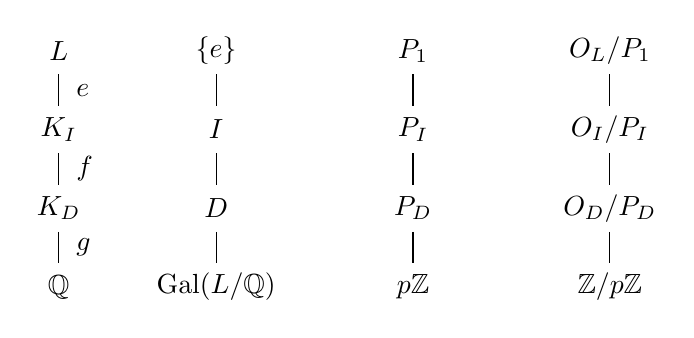
\begin{tikzpicture}[>=latex]
            \node at (0,-1) {$L$};
            \node at (2,-1) {$\bbrace{e}$};
            \node at (4.5,-1) {$P_1$};
            \node at (0,-2) {$K_{I}$};
            \node at (2,-2) {$I$};
            \node at (4.5,-2) {$P_{I}$};
            \node at (0,-3) {$K_{D}$};
            \node at (2,-3) {$D$};
            \node at (4.5,-3) {$P_{D}$};
            \node at (0,-4) {$\mathbb{Q}$};
            \node at (2,-4) {$\text{Gal}(L/\mathbb{Q})$};
            \node at (4.5,-4) {$p\mathbb{Z}$};
            \node at (7,-1)  {$O_{L}/P_1$};
            \node at (7,-2)  {$O_{I}/P_I$};
            \node at (7,-3)  {$O_{D}/P_D$};
            \node at (7,-4)  {$\mathbb{Z}/p\mathbb{Z}$};

            \draw (0,-1.3)--node[right=1mm]{$e$}(0,-1.7);
            \draw (0,-2.3)--node[right=1mm]{$f$}(0,-2.7);
            \draw (0,-3.3)--node[right=1mm]{$g$}(0,-3.7);
            \draw (2,-1.3)--(2,-1.7);
            \draw (2,-2.3)--(2,-2.7);
            \draw (2,-3.3)--(2,-3.7);
            \draw (4.5,-1.3)--(4.5,-1.7);
            \draw (4.5,-2.3)--(4.5,-2.7);
            \draw (4.5,-3.3)--(4.5,-3.7);
            \draw (7,-1.3)--(7,-1.7);
            \draw (7,-2.3)--(7,-2.7);
            \draw (7,-3.3)--(7,-3.7);
        \end{tikzpicture}
    \end{center}
    要证明$K_I$是$p\mathbb{Z}$的最大不分歧子域,考虑一个域$M$,$p\mathbb{Z}$在$M$上不分歧,则$p$在$MK_{I}$上不分歧,
    从而我们得到:\begin{equation*}
        [MK_I:\mathbb{Q}]=f\times (p\mathbb{Z}\,\text{在}MK_I\text{的分裂次数})\le f\times (p\mathbb{Z}\,\text{在}L\text{的分裂次数})=fg =[K_I:\mathbb{Q}]
    \end{equation*}
    从而$[MK_I:\mathbb{Q}]\le [K_I:\mathbb{Q}]\le [MK_I:\mathbb{Q}]$,证毕。


\end{prooff}

\section{理想类数与理想类群}
\subsection{类群与类数}
\begin{exer}
    设$A$是数域$K$的分式理想,求证:

    (a)$A$为整理想$\Leftrightarrow A\subseteq O_{k} $

    (b)$A^{-1}=\bbrace{\alpha \in K:\alpha A\subseteq O_{k}}$
\end{exer}
\begin{prooff}
    (a)的充分性显然,对于必要性,设$\mu A=I$,$I$为$O_{k}$中理想。直接按理想的定义验证$A$构成$O_{k}$中理想,
    比如$\forall x,y\in A$,$\mu(x+y)\in I=\mu A=$,从而$x+y\in A$

    (b)需要使用本书第二章第一节的引理5,对于$O_{k}$的非零理想$I$,以及其中非零元$\alpha\in I$,我们构造:
    \begin{equation*}
        J=\bbrace{\beta \in O_{k}:\beta I\subseteq (\alpha)}
    \end{equation*}
    从而有:$IJ=(\alpha)$,进而:
    \begin{equation*}
        A^{-1}=\frac{\mu}{\alpha}J=\bbrace{\frac{\mu}{\alpha}\beta :\beta\in O_{k},
            \frac{\mu \beta }{\alpha}A\subseteq O_{k}}=\bbrace{\gamma:\gamma\in K ,\gamma A\subseteq O_{k}}
    \end{equation*}

    上式最后一个等号左边包含右边是因为任意$\gamma\in K$,我们有:
    \begin{equation*}
        \beta = \frac{\alpha}{\mu }\gamma \in \gamma A \subseteq  O_{k}
    \end{equation*}
\end{prooff}

\begin{exer}
    $O_{k}$为主理想整环等价于$h(K)=1$
\end{exer}
\begin{prooff}
    只需证$O_{k}$为主理想整环,则所有分式理想为主分式理想,
    考虑分式理想$A=\frac{1}{\mu }I$,设$I=(\beta)$,则\begin{equation*}
        A=\frac{1}{\mu }I=\frac{1}{\mu }(\beta)=\frac{\beta}{\mu }O_k
    \end{equation*}
\end{prooff}
\begin{exer}
    设$a,b,c\in \mathbb{R}$,$4ac-b^2>0$,求证当$f\ge \frac{2}{\pi}\sqrt{4ac-b^2}$时,存在$(0,0)\neq (a,b)\in \mathbb{Z}^2$,使得$ax^2+bxy+cy^2\le f$
\end{exer}
\begin{prooff}
    考虑$\mathbb{R}^2$上的格$\mathbb{Z}^2$,其体积为$V(\mathbb{Z}^2)=1$,因此只需证明,关于原点对称的紧集\begin{equation*}
        A=\bbrace{(x,y)\in \mathbb{R}^2:ax^2+bxy+cy^2\le f}
    \end{equation*}
    的测度$\ge 4$.

    由于正交变换下,测度保持不变,对实对称矩阵$J=\begin{bmatrix}
            a           & \frac{b}{2} \\
            \frac{b}{2} & c
        \end{bmatrix}$用一个正交矩阵对角化得到$TJT^{-1}=\text{diag}(\lambda_1,\lambda_2)$,其中$\lambda_i,i=1,2$为方程$x^2-(a+c)x+ac-\frac{b^2}{4}$的两个根。

    从而
    \begin{equation*}
        \mu(A)=\mu(\bbrace{(x,y)\in \mathbb{R}^2:\lambda_1x^2+\lambda_2y^2\le f})=\frac{f\pi}{ \sqrt{\lambda_1\lambda_2}}\ge \frac{\frac{2}{\pi}\pi \sqrt{4ac-b^2}}{\sqrt{ac-\frac{b^2}{4}}}=4
    \end{equation*}
    由Minkowski定理命题得证。

\end{prooff}

\newpage
\section{部分细节补充}


% \pdfbookmark[1]{勘误}{勘误}
\section{勘误}
\begin{enumerate}
    \item 第28页引理3,将1改为$I$。
    \item 第42页定理2.7$(c)$,将$\mathfrak{p}$更正为$p$。
    \item 第50页第一行将最后一个等号的$\sum_{i=0}^{f-1}(\bar{\lambda})^{pi}$更正为$\sum_{i=0}^{f-1}(\bar{\lambda})^{p^i}$。
    \item 第56页3.2分解群与惯性群下第三行$\bar{K}=O_{K/\mathfrak{p}}$更正为$\bar{K}=O_{K}/\mathfrak{p}$。
    \item 第60页引理16(b)最后一个指数上的符号应为$f(\mathfrak{P}_{E}|\mathfrak{p})$。
    \item 第65页倒数第9行,将$\mathbb{F}p$更正为$\mathbb{F}_p$。
    \item 第69页第二行$\alpha$更正为$a$。
    \item 第107页习题6,将$p=1\mod{4}$更正为$p\equiv 1\mod{4}$,$d$更正为$p$。
    \item 
\end{enumerate}
\newpage
\bibliography{fkq}
\bibliographystyle{plain}%终端输入bibtex+文件名再ctrl+s两次



%\url{https://math.stackexchange.com/questions/4323}




\end{document}